\documentclass{beamer}
\usepackage[utf8]{inputenc}
\usetheme{Madrid}
\usepackage{tikz}
\usetikzlibrary{backgrounds}

\usepackage{mathpazo}

\newcounter{row}
\newcounter{col}

\newcommand\setrow[9]{
    \setcounter{col}{1}
    \foreach \n in {#1, #2, #3, #4, #5, #6, #7, #8, #9} {
        \edef\x{\value{col} - 0.5}
        \edef\y{9.5 - \value{row}}
        \node[digit,name={\arabic{row}-\arabic{col}}] at (\x, \y) {\n};
        \stepcounter{col}
    }
    \stepcounter{row}
}

\tikzset {
  hint/.style={blue, font=\sf, minimum width=3mm, minimum height=3mm},
  digit/.style = { minimum height = 5mm, minimum width=5mm, anchor=center }
}

\def\hintcell#1#2#3{
\node at (#1-#2) {\hintbox{#3}};
}

% UGLY code. Do not read :-)
\def\hintbox#1{
\resizebox{8.5mm}{8.5mm}{%
\tikz[scale=0.3]{%
  \def\auxc{0}
  \foreach \m in {1,...,9} {
    \pgfmathparse{mod(\auxc,3)}
    \xdef\x{\pgfmathresult}
    \pgfmathparse{-floor(\auxc/3)}
    \xdef\y{\pgfmathresult}
    \xdef\hintprinted{0}
    \foreach \n in {#1} {
      \ifnum\n=\m
       \node[hint] at (\x,\y) {\n};
       \xdef\hintprinted{1}
      \fi
     }
   \ifnum\hintprinted=0
      \node[hint, opacity=0.1] at (\x,\y) {\m};
   \fi
   \pgfmathparse{\auxc+1} 
   \xdef\auxc{\pgfmathresult}   }
  }%
  }
}

\title{Solving Sudoku as a Constraint Satisfaction Problem}

\author{Ingimar Örn Oddsson \& Johan Ejstrud}

% If you have a file called "university-logo-filename.xxx", where xxx
% is a graphic format that can be processed by latex or pdflatex,
% resp., then you can add a logo as follows:

% \pgfdeclareimage[height=1cm]{university-logo}{default_white}
% \logo{\pgfuseimage{university-logo}}

% Delete this, if you do not want the table of contents to pop up at
% the beginning of each subsection:
\AtBeginSubsection[]
{
  \begin{frame}<beamer>{Outline}
    \tableofcontents[currentsection,currentsubsection]
  \end{frame}
}

% Let's get started
\begin{document}

\begin{frame}
  \titlepage
\end{frame}

\begin{frame}
  \frametitle{Introduction}
  \begin{block}{Goals}
    \begin{itemize}
    \item Make a sudoku solver 
    \item Represent environment as constraint satisfaction problem
    \item Be able to handle different board sizes 
    \item Generate sudoku puzzles 
    \end{itemize}
  \end{block}

  \begin{block}{Motivation}
    \begin{itemize}
    \item Go deeper into CSP 
    \item Interesting handling general case  
    \end{itemize}
  \end{block}
\end{frame}

\begin{frame}
  \frametitle{Sudoku Rules}
    \begin{itemize}
    \item Each row contain all numbers from 1-9
    \item Each column contain all numbers from 1-9
    \item Block contain all numbers from 1-9
    \end{itemize}
  \begin{figure}
    \centering
  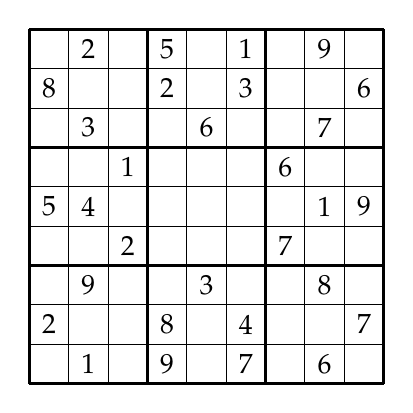
\begin{tikzpicture}[scale=.5]
    \draw (0, 0) grid (9, 9);
    \draw[very thick, scale=3] (0, 0) grid (3, 3);

    \setcounter{row}{1}
    \setrow { }{2}{ }  {5}{ }{1}  { }{9}{ }
    \setrow {8}{ }{ }  {2}{ }{3}  { }{ }{6}
    \setrow { }{3}{ }  { }{6}{ }  { }{7}{ }

    \setrow { }{ }{1}  { }{ }{ }  {6}{ }{ }
    \setrow {5}{4}{ }  { }{ }{ }  { }{1}{9}
    \setrow { }{ }{2}  { }{ }{ }  {7}{ }{ }

    \setrow { }{9}{ }  { }{3}{ }  { }{8}{ }
    \setrow {2}{ }{ }  {8}{ }{4}  { }{ }{7}
    \setrow { }{1}{ }  {9}{ }{7}  { }{6}{ }
  \end{tikzpicture}  
  \end{figure}
\end{frame}

\begin{frame}
  \frametitle{General Sudoku}
    \begin{itemize}
    \item Solve boards of size $n^2$, e.g $4 \times 4$, $16 \times 16$.
    \item Constraints cannot be hard-coded
    \end{itemize}
\end{frame}

\begin{frame}
  \frametitle{Constraints}
  \begin{block}{Initial Idea}
  \begin{itemize}
  \item Find way of generating constraints for any board size
  \item Add constraints to knowledge base 
  \end{itemize}    
  \end{block}

  \begin{figure}
    \centering
  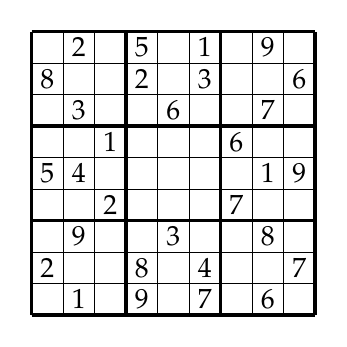
\begin{tikzpicture}[scale=.4]
    \draw (0, 0) grid (9, 9);
    \draw[very thick, scale=3] (0, 0) grid (3, 3);

    \setcounter{row}{1}
    \setrow { }{2}{ }  {5}{ }{1}  { }{9}{ }
    \setrow {8}{ }{ }  {2}{ }{3}  { }{ }{6}
    \setrow { }{3}{ }  { }{6}{ }  { }{7}{ }

    \setrow { }{ }{1}  { }{ }{ }  {6}{ }{ }
    \setrow {5}{4}{ }  { }{ }{ }  { }{1}{9}
    \setrow { }{ }{2}  { }{ }{ }  {7}{ }{ }

    \setrow { }{9}{ }  { }{3}{ }  { }{8}{ }
    \setrow {2}{ }{ }  {8}{ }{4}  { }{ }{7}
    \setrow { }{1}{ }  {9}{ }{7}  { }{6}{ }
  \end{tikzpicture}  
  \end{figure}
\end{frame}

\begin{frame}
  \frametitle{Constraints}
  \begin{block}{Number Of Constraints}
    \begin{itemize}
    \item 8+8+4 for each cell
    \item In total $\frac{(8+8+4)\cdot 81}{2} = 810$ constraints
    \item In general $\frac{(2 \cdot (n-1) + (n-1)^2) \cdot n^2}{2}$ constraints
    \item Quick increase e.g. $25 \times 25$ has 20000 constraints 
    \item Infeasible to generate constraints explicitly 
    \end{itemize}
  \end{block}

  \begin{figure}
    \centering
  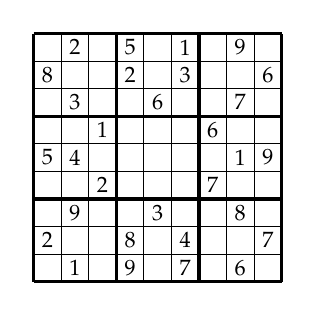
\begin{tikzpicture}[scale=.35]
    \footnotesize
    \draw (0, 0) grid (9, 9);
    \draw[very thick, scale=3] (0, 0) grid (3, 3);

    \setcounter{row}{1}
    \setrow { }{2}{ }  {5}{ }{1}  { }{9}{ }
    \setrow {8}{ }{ }  {2}{ }{3}  { }{ }{6}
    \setrow { }{3}{ }  { }{6}{ }  { }{7}{ }

    \setrow { }{ }{1}  { }{ }{ }  {6}{ }{ }
    \setrow {5}{4}{ }  { }{ }{ }  { }{1}{9}
    \setrow { }{ }{2}  { }{ }{ }  {7}{ }{ }

    \setrow { }{9}{ }  { }{3}{ }  { }{8}{ }
    \setrow {2}{ }{ }  {8}{ }{4}  { }{ }{7}
    \setrow { }{1}{ }  {9}{ }{7}  { }{6}{ }
  \end{tikzpicture}  
  \end{figure}
\end{frame}

\begin{frame}
  \frametitle{Initializing Sudoku}
    \begin{itemize}
    \item Module constraints implicitly 
    \item Each cell is a variable
    \item The domain of each variable is updated
    \item Add initial numbers one by one
    \end{itemize}
\end{frame}

\begin{frame}
  \frametitle{Initializing Sudoku}
  \begin{figure}
    \centering
  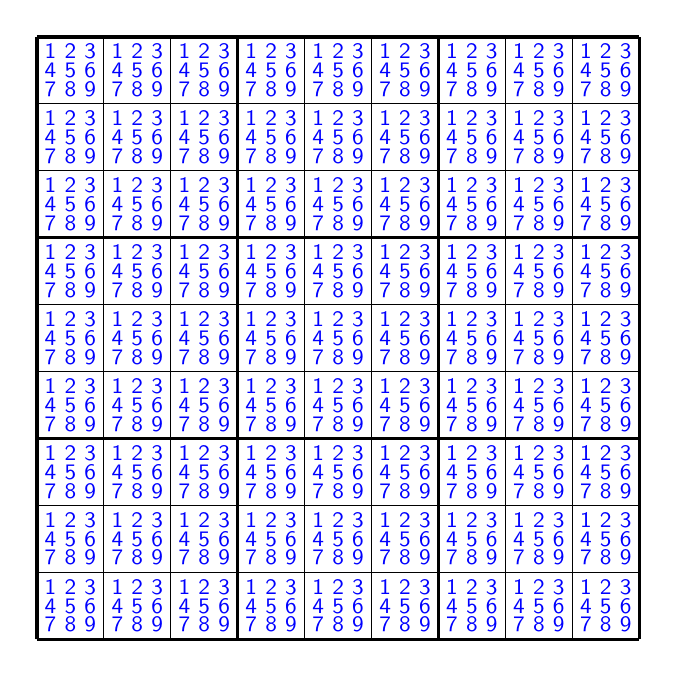
\begin{tikzpicture}[scale=.85]
  \begin{scope}
    \draw (0, 0) grid (9, 9);
    \draw[very thick, scale=3] (0, 0) grid (3, 3);

    \setcounter{row}{1}
    \setrow { }{ }{ }  { }{ }{ }  { }{ }{ }
    \setrow { }{ }{ }  { }{ }{ }  { }{ }{ }
    \setrow { }{ }{ }  { }{ }{ }  { }{ }{ }

    \setrow { }{ }{ }  { }{ }{ }  { }{ }{ }
    \setrow { }{ }{ }  { }{ }{ }  { }{ }{ }
    \setrow { }{ }{ }  { }{ }{ }  { }{ }{ }

    \setrow { }{ }{ }  { }{ }{ }  { }{ }{ }
    \setrow { }{ }{ }  { }{ }{ }  { }{ }{ }
    \setrow { }{ }{ }  { }{ }{ }  { }{ }{ }

    % Hints
    \hintcell{1}{1}{1,2,3,4,5,6,7,8,9}
    \hintcell{1}{2}{1,2,3,4,5,6,7,8,9}
    \hintcell{1}{3}{1,2,3,4,5,6,7,8,9}
    \hintcell{1}{4}{1,2,3,4,5,6,7,8,9}
    \hintcell{1}{5}{1,2,3,4,5,6,7,8,9}
    \hintcell{1}{6}{1,2,3,4,5,6,7,8,9}
    \hintcell{1}{7}{1,2,3,4,5,6,7,8,9}
    \hintcell{1}{8}{1,2,3,4,5,6,7,8,9}
    \hintcell{1}{9}{1,2,3,4,5,6,7,8,9}
    \hintcell{2}{1}{1,2,3,4,5,6,7,8,9}
    \hintcell{2}{2}{1,2,3,4,5,6,7,8,9}
    \hintcell{2}{3}{1,2,3,4,5,6,7,8,9}
    \hintcell{2}{4}{1,2,3,4,5,6,7,8,9}
    \hintcell{2}{5}{1,2,3,4,5,6,7,8,9}
    \hintcell{2}{6}{1,2,3,4,5,6,7,8,9}
    \hintcell{2}{7}{1,2,3,4,5,6,7,8,9}
    \hintcell{2}{8}{1,2,3,4,5,6,7,8,9}
    \hintcell{2}{9}{1,2,3,4,5,6,7,8,9}
    \hintcell{3}{1}{1,2,3,4,5,6,7,8,9}
    \hintcell{3}{2}{1,2,3,4,5,6,7,8,9}
    \hintcell{3}{3}{1,2,3,4,5,6,7,8,9}
    \hintcell{3}{4}{1,2,3,4,5,6,7,8,9}
    \hintcell{3}{5}{1,2,3,4,5,6,7,8,9}
    \hintcell{3}{6}{1,2,3,4,5,6,7,8,9}
    \hintcell{3}{7}{1,2,3,4,5,6,7,8,9}
    \hintcell{3}{8}{1,2,3,4,5,6,7,8,9}
    \hintcell{3}{9}{1,2,3,4,5,6,7,8,9}
    \hintcell{4}{1}{1,2,3,4,5,6,7,8,9}
    \hintcell{4}{2}{1,2,3,4,5,6,7,8,9}
    \hintcell{4}{3}{1,2,3,4,5,6,7,8,9}
    \hintcell{4}{4}{1,2,3,4,5,6,7,8,9}
    \hintcell{4}{5}{1,2,3,4,5,6,7,8,9}
    \hintcell{4}{6}{1,2,3,4,5,6,7,8,9}
    \hintcell{4}{7}{1,2,3,4,5,6,7,8,9}
    \hintcell{4}{8}{1,2,3,4,5,6,7,8,9}
    \hintcell{4}{9}{1,2,3,4,5,6,7,8,9}
    \hintcell{5}{1}{1,2,3,4,5,6,7,8,9}
    \hintcell{5}{2}{1,2,3,4,5,6,7,8,9}
    \hintcell{5}{3}{1,2,3,4,5,6,7,8,9}
    \hintcell{5}{4}{1,2,3,4,5,6,7,8,9}
    \hintcell{5}{5}{1,2,3,4,5,6,7,8,9}
    \hintcell{5}{6}{1,2,3,4,5,6,7,8,9}
    \hintcell{5}{7}{1,2,3,4,5,6,7,8,9}
    \hintcell{5}{8}{1,2,3,4,5,6,7,8,9}
    \hintcell{5}{9}{1,2,3,4,5,6,7,8,9}
    \hintcell{6}{1}{1,2,3,4,5,6,7,8,9}
    \hintcell{6}{2}{1,2,3,4,5,6,7,8,9}
    \hintcell{6}{3}{1,2,3,4,5,6,7,8,9}
    \hintcell{6}{4}{1,2,3,4,5,6,7,8,9}
    \hintcell{6}{5}{1,2,3,4,5,6,7,8,9}
    \hintcell{6}{6}{1,2,3,4,5,6,7,8,9}
    \hintcell{6}{7}{1,2,3,4,5,6,7,8,9}
    \hintcell{6}{8}{1,2,3,4,5,6,7,8,9}
    \hintcell{6}{9}{1,2,3,4,5,6,7,8,9}
    \hintcell{7}{1}{1,2,3,4,5,6,7,8,9}
    \hintcell{7}{2}{1,2,3,4,5,6,7,8,9}
    \hintcell{7}{3}{1,2,3,4,5,6,7,8,9}
    \hintcell{7}{4}{1,2,3,4,5,6,7,8,9}
    \hintcell{7}{5}{1,2,3,4,5,6,7,8,9}
    \hintcell{7}{6}{1,2,3,4,5,6,7,8,9}
    \hintcell{7}{7}{1,2,3,4,5,6,7,8,9}
    \hintcell{7}{8}{1,2,3,4,5,6,7,8,9}
    \hintcell{7}{9}{1,2,3,4,5,6,7,8,9}
    \hintcell{8}{1}{1,2,3,4,5,6,7,8,9}
    \hintcell{8}{2}{1,2,3,4,5,6,7,8,9}
    \hintcell{8}{3}{1,2,3,4,5,6,7,8,9}
    \hintcell{8}{4}{1,2,3,4,5,6,7,8,9}
    \hintcell{8}{5}{1,2,3,4,5,6,7,8,9}
    \hintcell{8}{6}{1,2,3,4,5,6,7,8,9}
    \hintcell{8}{7}{1,2,3,4,5,6,7,8,9}
    \hintcell{8}{8}{1,2,3,4,5,6,7,8,9}
    \hintcell{8}{9}{1,2,3,4,5,6,7,8,9}
    \hintcell{9}{1}{1,2,3,4,5,6,7,8,9}
    \hintcell{9}{2}{1,2,3,4,5,6,7,8,9}
    \hintcell{9}{3}{1,2,3,4,5,6,7,8,9}
    \hintcell{9}{4}{1,2,3,4,5,6,7,8,9}
    \hintcell{9}{5}{1,2,3,4,5,6,7,8,9}
    \hintcell{9}{6}{1,2,3,4,5,6,7,8,9}
    \hintcell{9}{7}{1,2,3,4,5,6,7,8,9}
    \hintcell{9}{8}{1,2,3,4,5,6,7,8,9}
    \hintcell{9}{9}{1,2,3,4,5,6,7,8,9}
  \end{scope}
\end{tikzpicture}
\end{figure}
\end{frame}

\begin{frame}
  \frametitle{Initializing Sudoku}
  \begin{figure}
    \centering
  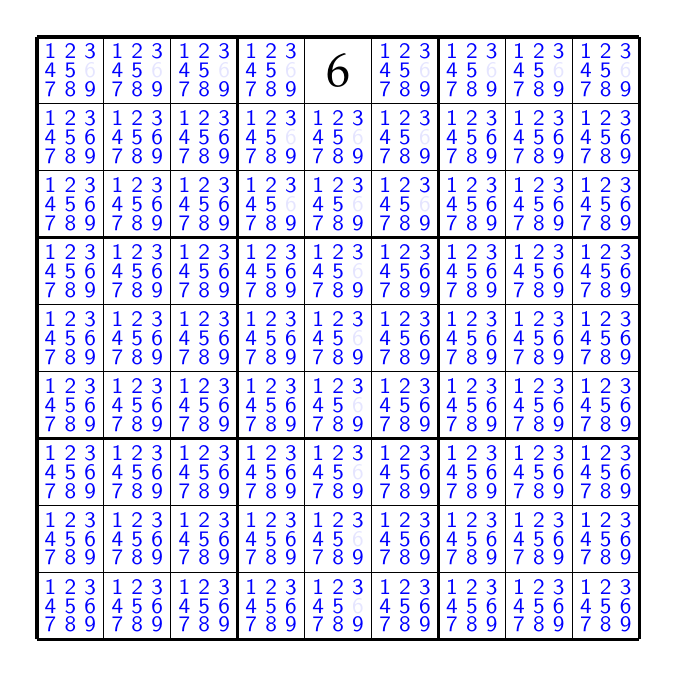
\begin{tikzpicture}[scale=.85]
  \begin{scope}
    \LARGE
    \draw (0, 0) grid (9, 9);
    \draw[very thick, scale=3] (0, 0) grid (3, 3);

    \setcounter{row}{1}
    \setrow { }{ }{ }  { }{6}{ }  { }{ }{ }
    \setrow { }{ }{ }  { }{ }{ }  { }{ }{ }
    \setrow { }{ }{ }  { }{ }{ }  { }{ }{ }

    \setrow { }{ }{ }  { }{ }{ }  { }{ }{ }
    \setrow { }{ }{ }  { }{ }{ }  { }{ }{ }
    \setrow { }{ }{ }  { }{ }{ }  { }{ }{ }

    \setrow { }{ }{ }  { }{ }{ }  { }{ }{ }
    \setrow { }{ }{ }  { }{ }{ }  { }{ }{ }
    \setrow { }{ }{ }  { }{ }{ }  { }{ }{ }
    
    \normalsize
    % Hints
    \hintcell{1}{1}{1,2,3,4,5,7,8,9}
    \hintcell{1}{2}{1,2,3,4,5,7,8,9}
    \hintcell{1}{3}{1,2,3,4,5,7,8,9}
    \hintcell{1}{4}{1,2,3,4,5,7,8,9}
    \hintcell{1}{6}{1,2,3,4,5,7,8,9}
    \hintcell{1}{7}{1,2,3,4,5,7,8,9}
    \hintcell{1}{8}{1,2,3,4,5,7,8,9}
    \hintcell{1}{9}{1,2,3,4,5,7,8,9}
    \hintcell{2}{1}{1,2,3,4,5,6,7,8,9}
    \hintcell{2}{2}{1,2,3,4,5,6,7,8,9}
    \hintcell{2}{3}{1,2,3,4,5,6,7,8,9}
    \hintcell{2}{4}{1,2,3,4,5,7,8,9}
    \hintcell{2}{5}{1,2,3,4,5,7,8,9}
    \hintcell{2}{6}{1,2,3,4,5,7,8,9}
    \hintcell{2}{7}{1,2,3,4,5,6,7,8,9}
    \hintcell{2}{8}{1,2,3,4,5,6,7,8,9}
    \hintcell{2}{9}{1,2,3,4,5,6,7,8,9}
    \hintcell{3}{1}{1,2,3,4,5,6,7,8,9}
    \hintcell{3}{2}{1,2,3,4,5,6,7,8,9}
    \hintcell{3}{3}{1,2,3,4,5,6,7,8,9}
    \hintcell{3}{4}{1,2,3,4,5,7,8,9}
    \hintcell{3}{5}{1,2,3,4,5,7,8,9}
    \hintcell{3}{6}{1,2,3,4,5,7,8,9}
    \hintcell{3}{7}{1,2,3,4,5,6,7,8,9}
    \hintcell{3}{8}{1,2,3,4,5,6,7,8,9}
    \hintcell{3}{9}{1,2,3,4,5,6,7,8,9}
    \hintcell{4}{1}{1,2,3,4,5,6,7,8,9}
    \hintcell{4}{2}{1,2,3,4,5,6,7,8,9}
    \hintcell{4}{3}{1,2,3,4,5,6,7,8,9}
    \hintcell{4}{4}{1,2,3,4,5,6,7,8,9}
    \hintcell{4}{5}{1,2,3,4,5,7,8,9}
    \hintcell{4}{6}{1,2,3,4,5,6,7,8,9}
    \hintcell{4}{7}{1,2,3,4,5,6,7,8,9}
    \hintcell{4}{8}{1,2,3,4,5,6,7,8,9}
    \hintcell{4}{9}{1,2,3,4,5,6,7,8,9}
    \hintcell{5}{1}{1,2,3,4,5,6,7,8,9}
    \hintcell{5}{2}{1,2,3,4,5,6,7,8,9}
    \hintcell{5}{3}{1,2,3,4,5,6,7,8,9}
    \hintcell{5}{4}{1,2,3,4,5,6,7,8,9}
    \hintcell{5}{5}{1,2,3,4,5,7,8,9}
    \hintcell{5}{6}{1,2,3,4,5,6,7,8,9}
    \hintcell{5}{7}{1,2,3,4,5,6,7,8,9}
    \hintcell{5}{8}{1,2,3,4,5,6,7,8,9}
    \hintcell{5}{9}{1,2,3,4,5,6,7,8,9}
    \hintcell{6}{1}{1,2,3,4,5,6,7,8,9}
    \hintcell{6}{2}{1,2,3,4,5,6,7,8,9}
    \hintcell{6}{3}{1,2,3,4,5,6,7,8,9}
    \hintcell{6}{4}{1,2,3,4,5,6,7,8,9}
    \hintcell{6}{5}{1,2,3,4,5,7,8,9}
    \hintcell{6}{6}{1,2,3,4,5,6,7,8,9}
    \hintcell{6}{7}{1,2,3,4,5,6,7,8,9}
    \hintcell{6}{8}{1,2,3,4,5,6,7,8,9}
    \hintcell{6}{9}{1,2,3,4,5,6,7,8,9}
    \hintcell{7}{1}{1,2,3,4,5,6,7,8,9}
    \hintcell{7}{2}{1,2,3,4,5,6,7,8,9}
    \hintcell{7}{3}{1,2,3,4,5,6,7,8,9}
    \hintcell{7}{4}{1,2,3,4,5,6,7,8,9}
    \hintcell{7}{5}{1,2,3,4,5,7,8,9}
    \hintcell{7}{6}{1,2,3,4,5,6,7,8,9}
    \hintcell{7}{7}{1,2,3,4,5,6,7,8,9}
    \hintcell{7}{8}{1,2,3,4,5,6,7,8,9}
    \hintcell{7}{9}{1,2,3,4,5,6,7,8,9}
    \hintcell{8}{1}{1,2,3,4,5,6,7,8,9}
    \hintcell{8}{2}{1,2,3,4,5,6,7,8,9}
    \hintcell{8}{3}{1,2,3,4,5,6,7,8,9}
    \hintcell{8}{4}{1,2,3,4,5,6,7,8,9}
    \hintcell{8}{5}{1,2,3,4,5,7,8,9}
    \hintcell{8}{6}{1,2,3,4,5,6,7,8,9}
    \hintcell{8}{7}{1,2,3,4,5,6,7,8,9}
    \hintcell{8}{8}{1,2,3,4,5,6,7,8,9}
    \hintcell{8}{9}{1,2,3,4,5,6,7,8,9}
    \hintcell{9}{1}{1,2,3,4,5,6,7,8,9}
    \hintcell{9}{2}{1,2,3,4,5,6,7,8,9}
    \hintcell{9}{3}{1,2,3,4,5,6,7,8,9}
    \hintcell{9}{4}{1,2,3,4,5,6,7,8,9}
    \hintcell{9}{5}{1,2,3,4,5,7,8,9}
    \hintcell{9}{6}{1,2,3,4,5,6,7,8,9}
    \hintcell{9}{7}{1,2,3,4,5,6,7,8,9}
    \hintcell{9}{8}{1,2,3,4,5,6,7,8,9}
    \hintcell{9}{9}{1,2,3,4,5,6,7,8,9}
  \end{scope}
\end{tikzpicture}
\end{figure}
\end{frame}

\begin{frame}
  \frametitle{Initializing Sudoku}
  \begin{figure}
    \centering
  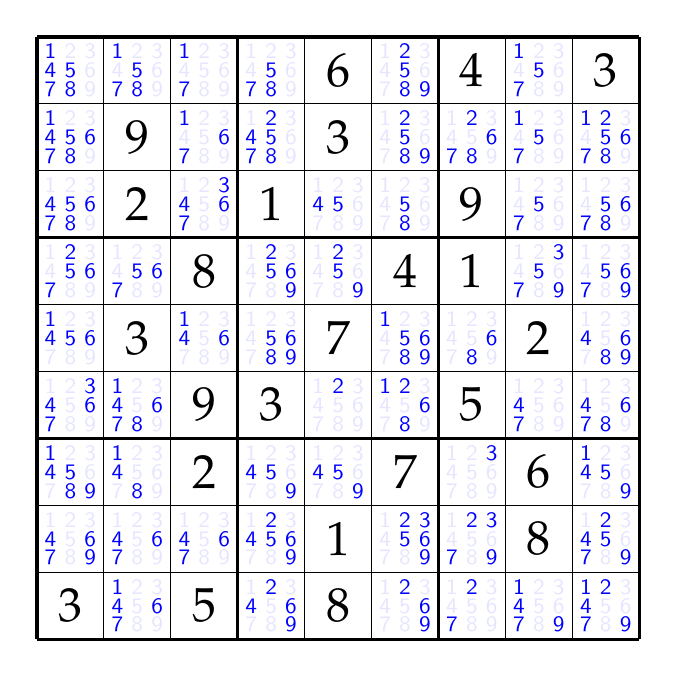
\begin{tikzpicture}[scale=.85]
  \begin{scope}
    \LARGE
    \draw (0, 0) grid (9, 9);
    \draw[very thick, scale=3] (0, 0) grid (3, 3);

    \setcounter{row}{1}
    \setrow { }{ }{ }  { }{6}{ }  {4}{ }{3}
    \setrow { }{9}{ }  { }{3}{ }  { }{ }{ }
    \setrow { }{2}{ }  {1}{ }{ }  {9}{ }{ }

    \setrow { }{ }{8}  { }{ }{4}  {1}{ }{ }
    \setrow { }{3}{ }  { }{7}{ }  { }{2}{ }
    \setrow { }{ }{9}  {3}{ }{ }  {5}{ }{ }

    \setrow { }{ }{2}  { }{ }{7}  { }{6}{ }
    \setrow { }{ }{ }  { }{1}{ }  { }{8}{ }
    \setrow {3}{ }{5}  { }{8}{ }  { }{ }{ }
    
    \normalsize
    % Hints
    \hintcell{1}{1}{1,4,5,7,8}
    \hintcell{1}{2}{1,5,7,8}
    \hintcell{1}{3}{1,7}
    \hintcell{1}{4}{5,7,8}
    \hintcell{1}{6}{2,5,8,9}
    \hintcell{1}{8}{1,5,7}
    \hintcell{2}{1}{1,4,5,6,7,8}
    \hintcell{2}{3}{1,6,7}
    \hintcell{2}{4}{2,4,5,7,8}
    \hintcell{2}{6}{2,5,8,9}
    \hintcell{2}{7}{2,6,7,8}
    \hintcell{2}{8}{1,5,7}
    \hintcell{2}{9}{1,2,5,6,7,8}
    \hintcell{3}{1}{4,5,6,7,8}
    \hintcell{3}{3}{3,4,6,7}
    \hintcell{3}{5}{4,5}
    \hintcell{3}{6}{5,8}
    \hintcell{3}{8}{5,7}
    \hintcell{3}{9}{5,6,7,8}
    \hintcell{4}{1}{2,5,6,7}
    \hintcell{4}{2}{5,6,7}
    \hintcell{4}{4}{2,5,6,9}
    \hintcell{4}{5}{2,5,9}
    \hintcell{4}{8}{3,5,7,9}
    \hintcell{4}{9}{5,6,7,9}
    \hintcell{5}{1}{1,4,5,6}
    \hintcell{5}{3}{1,4,6}
    \hintcell{5}{4}{5,6,8,9}
    \hintcell{5}{6}{1,5,6,8,9}
    \hintcell{5}{7}{6,8}
    \hintcell{5}{9}{4,6,8,9}
    \hintcell{6}{1}{3,4,6,7}
    \hintcell{6}{2}{1,4,6,7,8}
    \hintcell{6}{5}{2}
    \hintcell{6}{6}{1,2,6,8}
    \hintcell{6}{8}{4,7}
    \hintcell{6}{9}{4,6,7,8}
    \hintcell{7}{1}{1,4,5,8,9}
    \hintcell{7}{2}{1,4,8}
    \hintcell{7}{4}{4,5,9}
    \hintcell{7}{5}{4,5,9}
    \hintcell{7}{7}{3}
    \hintcell{7}{9}{1,4,5,9}
    \hintcell{8}{1}{4,6,7,9}
    \hintcell{8}{2}{4,6,7}
    \hintcell{8}{3}{4,6,7}
    \hintcell{8}{4}{2,4,5,6,9}
    \hintcell{8}{6}{2,3,5,6,9}
    \hintcell{8}{7}{2,3,7,9}
    \hintcell{8}{9}{2,4,5,7,9}
    \hintcell{9}{2}{1,4,6,7}
    \hintcell{9}{4}{2,4,6,9}
    \hintcell{9}{6}{2,6,9}
    \hintcell{9}{7}{2,7}
    \hintcell{9}{8}{1,4,7,9}
    \hintcell{9}{9}{1,2,4,7,9}
  \end{scope}
\end{tikzpicture}
\end{figure}
\end{frame}

\begin{frame}
  \frametitle{Solving the Sudoku}
  \begin{itemize}
  \item Take most constrained variable
  \item Take most constraining variable
  \item Take least constraining value
  \end{itemize}
\end{frame}

\begin{frame}
  \frametitle{Solving the Sudoku}
  \begin{figure}
    \centering
  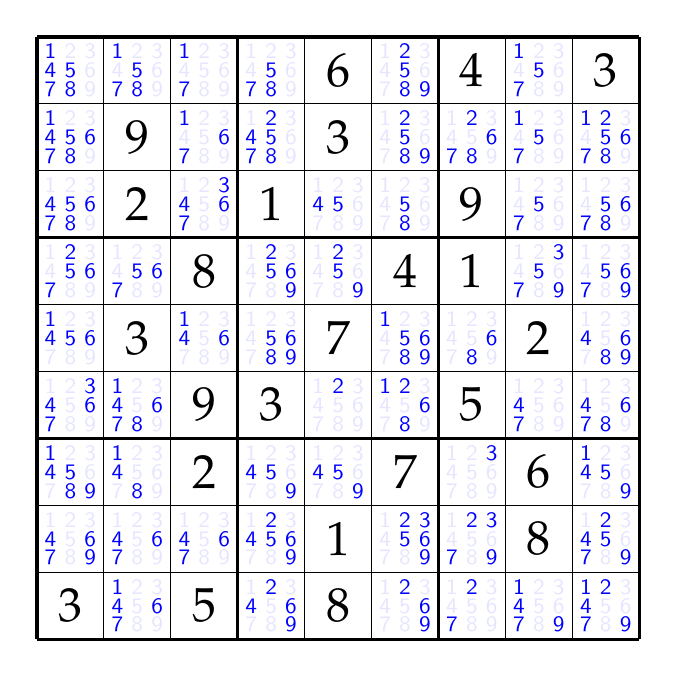
\begin{tikzpicture}[scale=.85]
  \begin{scope}
    \LARGE
    \draw (0, 0) grid (9, 9);
    \draw[very thick, scale=3] (0, 0) grid (3, 3);

    \setcounter{row}{1}
    \setrow { }{ }{ }  { }{6}{ }  {4}{ }{3}
    \setrow { }{9}{ }  { }{3}{ }  { }{ }{ }
    \setrow { }{2}{ }  {1}{ }{ }  {9}{ }{ }

    \setrow { }{ }{8}  { }{ }{4}  {1}{ }{ }
    \setrow { }{3}{ }  { }{7}{ }  { }{2}{ }
    \setrow { }{ }{9}  {3}{ }{ }  {5}{ }{ }

    \setrow { }{ }{2}  { }{ }{7}  { }{6}{ }
    \setrow { }{ }{ }  { }{1}{ }  { }{8}{ }
    \setrow {3}{ }{5}  { }{8}{ }  { }{ }{ }
    
    \normalsize
    % Hints
    \hintcell{1}{1}{1,4,5,7,8}
    \hintcell{1}{2}{1,5,7,8}
    \hintcell{1}{3}{1,7}
    \hintcell{1}{4}{5,7,8}
    \hintcell{1}{6}{2,5,8,9}
    \hintcell{1}{8}{1,5,7}
    \hintcell{2}{1}{1,4,5,6,7,8}
    \hintcell{2}{3}{1,6,7}
    \hintcell{2}{4}{2,4,5,7,8}
    \hintcell{2}{6}{2,5,8,9}
    \hintcell{2}{7}{2,6,7,8}
    \hintcell{2}{8}{1,5,7}
    \hintcell{2}{9}{1,2,5,6,7,8}
    \hintcell{3}{1}{4,5,6,7,8}
    \hintcell{3}{3}{3,4,6,7}
    \hintcell{3}{5}{4,5}
    \hintcell{3}{6}{5,8}
    \hintcell{3}{8}{5,7}
    \hintcell{3}{9}{5,6,7,8}
    \hintcell{4}{1}{2,5,6,7}
    \hintcell{4}{2}{5,6,7}
    \hintcell{4}{4}{2,5,6,9}
    \hintcell{4}{5}{2,5,9}
    \hintcell{4}{8}{3,5,7,9}
    \hintcell{4}{9}{5,6,7,9}
    \hintcell{5}{1}{1,4,5,6}
    \hintcell{5}{3}{1,4,6}
    \hintcell{5}{4}{5,6,8,9}
    \hintcell{5}{6}{1,5,6,8,9}
    \hintcell{5}{7}{6,8}
    \hintcell{5}{9}{4,6,8,9}
    \hintcell{6}{1}{3,4,6,7}
    \hintcell{6}{2}{1,4,6,7,8}
    \hintcell{6}{5}{2}
    \hintcell{6}{6}{1,2,6,8}
    \hintcell{6}{8}{4,7}
    \hintcell{6}{9}{4,6,7,8}
    \hintcell{7}{1}{1,4,5,8,9}
    \hintcell{7}{2}{1,4,8}
    \hintcell{7}{4}{4,5,9}
    \hintcell{7}{5}{4,5,9}
    \hintcell{7}{7}{3}
    \hintcell{7}{9}{1,4,5,9}
    \hintcell{8}{1}{4,6,7,9}
    \hintcell{8}{2}{4,6,7}
    \hintcell{8}{3}{4,6,7}
    \hintcell{8}{4}{2,4,5,6,9}
    \hintcell{8}{6}{2,3,5,6,9}
    \hintcell{8}{7}{2,3,7,9}
    \hintcell{8}{9}{2,4,5,7,9}
    \hintcell{9}{2}{1,4,6,7}
    \hintcell{9}{4}{2,4,6,9}
    \hintcell{9}{6}{2,6,9}
    \hintcell{9}{7}{2,7}
    \hintcell{9}{8}{1,4,7,9}
    \hintcell{9}{9}{1,2,4,7,9}
  \end{scope}
\end{tikzpicture}
\end{figure}
\end{frame}

\begin{frame}
  \frametitle{Conclusion}
  \begin{itemize}
  \item Our script successfully solves sudokus 
  \item Speed
\begin{table}[]
\centering
\label{my-label}
\begin{tabular}{c|c|c}
\textbf{Size }        &\textbf{ Difficulty }& \textbf{Time (ms)} \\ \hline
$4 \times 4$ & Hard       & 1         \\ \hline
$9 \times 9$ & Easy       & 8         \\ \hline
$9 \times 9$ & Evil       & 45        \\ \hline
$16 \times 16$ & Evil     & 80908     \\ 
\end{tabular}
\end{table}
  \end{itemize}
\end{frame}

\begin{frame}
  \frametitle{Future Work}
  \begin{block}{Sudoku Generator}
    \begin{itemize}
    \item Use solver to make generator 
    \item Unique solution
    \end{itemize}
  \end{block}
\end{frame}

\end{document}

%%% Local Variables:
%%% mode: latex
%%% TeX-master: t
%%% End:
